\documentclass[12pt,a4paper]{article}

% ─── Page Layout ───────────────────────────────────────────────────────────────
\usepackage[a4paper, margin=0.8in, headheight=14pt]{geometry}

% ─── Fonts (XeLaTeX) ───────────────────────────────────────────────────────────
\usepackage{fontspec}
\usepackage{unicode-math}
\setmainfont{TeX Gyre Pagella}
\setmonofont[Scale=0.88]{TeX Gyre Cursor}
\setmathfont{Latin Modern Math}

% ─── Packages ──────────────────────────────────────────────────────────────────
\usepackage{xcolor}
\usepackage{colortbl}
\usepackage{titlesec}
\usepackage{enumitem}
\usepackage{tabularx}
\usepackage{booktabs}
\usepackage{array}
\usepackage{amsmath}
\usepackage{tikz}
\usetikzlibrary{shapes.geometric, arrows.meta, positioning, calc, fit, decorations.pathreplacing, patterns}
\usepackage{tcolorbox}
\tcbuselibrary{skins, breakable}
\usepackage{hyperref}
\usepackage{fancyhdr}
\usepackage{graphicx}
\usepackage{microtype}
\hyphenpenalty=10000
\exhyphenpenalty=10000
\sloppy
\usepackage{caption}
\usepackage{setspace}
\usepackage{multirow}
\usepackage{tocloft}

% ─── Q&A helper ────────────────────────────────────────────────────────────────
\newcommand{\Q}[1]{\textbf{#1}\par\noindent\ignorespaces}

% ─── Colour Palette ────────────────────────────────────────────────────────────
\definecolor{myred}{RGB}{196,30,58}
\definecolor{mydark}{RGB}{30,30,50}
\definecolor{mygreen}{RGB}{14,120,80}
\definecolor{myteal}{RGB}{0,130,140}
\definecolor{myamber}{RGB}{180,100,0}
\definecolor{mypurple}{RGB}{100,30,160}
\definecolor{mygray}{RGB}{246,247,249}
\definecolor{mgframe}{RGB}{180,185,200}
\definecolor{watermark}{RGB}{145,150,170}
\definecolor{hdrred}{RGB}{250,232,235}
\definecolor{hdrgreen}{RGB}{220,244,233}
\definecolor{hdrteal}{RGB}{220,242,244}
\definecolor{hdramber}{RGB}{253,242,215}
\definecolor{hdrpurple}{RGB}{238,228,255}
\definecolor{hdrgray}{RGB}{238,240,245}
\definecolor{rowalt}{RGB}{250,251,253}

% ─── Section Formatting ────────────────────────────────────────────────────────
\titleformat{\section}
  {\large\bfseries\color{myred}}{\thesection.}{0.5em}{}
  [\vspace{1pt}{\color{myred}\rule{\linewidth}{0.8pt}}]
\titleformat{\subsection}
  {\normalsize\bfseries\color{myteal}}{\thesubsection}{0.5em}{}
\titlespacing*{\section}{0pt}{18pt}{7pt}
\titlespacing*{\subsection}{0pt}{11pt}{4pt}

% ─── Paragraph ─────────────────────────────────────────────────────────────────
\setlength{\parindent}{0pt}
\setlength{\parskip}{4pt}

% ─── TOC Styling ───────────────────────────────────────────────────────────────
\renewcommand{\cfttoctitlefont}{\large\bfseries\color{myred}}
\renewcommand{\cftaftertoctitle}{\par\noindent{\color{myred}\rule{\linewidth}{0.8pt}}}
\setlength{\cftbeforetoctitleskip}{0pt}
\setlength{\cftaftertoctitleskip}{6pt}
\renewcommand{\cftsecfont}{\normalsize\bfseries\color{mydark}}
\renewcommand{\cftsecpagefont}{\normalsize\bfseries\color{mydark}}
\renewcommand{\cftsecleader}{\cftdotfill{\cftdotsep}}
\setlength{\cftbeforesecskip}{7pt}
\renewcommand{\cftsubsecfont}{\small\color{mydark}}
\renewcommand{\cftsubsecpagefont}{\small\color{mydark}}
\setlength{\cftbeforesubsecskip}{3pt}
\setlength{\cftsubsecindent}{1.4em}

% ─── Table helpers ─────────────────────────────────────────────────────────────
\renewcommand{\arraystretch}{1.45}
\setlength{\tabcolsep}{6pt}
\arrayrulecolor{mydark}
\newcolumntype{B}[1]{>{\small\bfseries\raggedright\arraybackslash}m{#1}}
\newcolumntype{Y}{>{\small\raggedright\arraybackslash}X}
\renewcommand{\tabularxcolumn}[1]{m{#1}}

% ─── Header / Footer ───────────────────────────────────────────────────────────
\pagestyle{fancy}
\fancyhf{}
\fancyhead[L]{\small\color{myred}\textbf{EC304}\;\color{mydark}--- Network Theory}
\fancyhead[R]{\small\color{myteal}\textbf{Module 2 Notes}}
\fancyfoot[C]{\small\color{mydark}\thepage}
\fancyfoot[R]{\small\color{watermark}\textit{\copyright\ Biraj}}
\renewcommand{\headrulewidth}{0.5pt}
\renewcommand{\footrulewidth}{0.3pt}

% ─── Hyperref ──────────────────────────────────────────────────────────────────
\hypersetup{
  colorlinks=true, linkcolor=myteal, urlcolor=myteal,
  pdfauthor={Biraj Sarkar (CGEC)},
  pdftitle={EC304 --- Module 2 Notes: Fourier Analysis and Three-Phase Unbalanced Systems}
}

% ─── tcolorbox styles ──────────────────────────────────────────────────────────
\tcbset{
  tikzbox/.style={
    colback=mygray, colframe=mgframe, boxrule=0.6pt, arc=4pt,
    left=8pt, right=8pt, top=6pt, bottom=6pt,
    colbacktitle=mgframe, coltitle=mydark,
    fonttitle=\small\bfseries
  },
  defbox/.style={
    colback=hdrgreen, colframe=mygreen, boxrule=0.8pt, arc=4pt,
    left=9pt, right=9pt, top=6pt, bottom=6pt,
    colbacktitle=mygreen, coltitle=white,
    fonttitle=\small\bfseries
  },
  formulabox/.style={
    colback=hdrteal, colframe=myteal, boxrule=0.8pt, arc=4pt,
    left=9pt, right=9pt, top=7pt, bottom=7pt,
    colbacktitle=myteal, coltitle=white,
    fonttitle=\small\bfseries
  },
  examplebox/.style={
    colback=hdramber, colframe=myamber, boxrule=0.8pt, arc=4pt,
    left=9pt, right=9pt, top=6pt, bottom=6pt,
    colbacktitle=myamber, coltitle=white,
    fonttitle=\small\bfseries
  },
  masonbox/.style={
    colback=hdrpurple, colframe=mypurple, boxrule=0.8pt, arc=4pt,
    left=9pt, right=9pt, top=6pt, bottom=6pt,
    colbacktitle=mypurple, coltitle=white,
    fonttitle=\small\bfseries
  },
  exambox/.style={
    colback=hdrpurple, colframe=mypurple, boxrule=1pt, arc=5pt,
    left=10pt, right=10pt, top=8pt, bottom=8pt,
    colbacktitle=mypurple, coltitle=white,
    fonttitle=\bfseries,
    breakable, title after break={\textbf{Frequently Asked / Viva Questions (contd.)}}
  }
}
\tcbset{breakable}
\tcbset{after={\color{black}}}

% ─── TikZ styles ───────────────────────────────────────────────────────────────
\tikzset{
  circnode/.style={circle, draw=myteal, fill=hdrteal, inner sep=2pt, minimum size=6pt},
  block/.style={rectangle, draw=myteal, fill=hdrteal, text width=2.4cm, align=center, minimum height=0.95cm, font=\small, rounded corners=3pt, line width=0.7pt},
  arrow/.style={-Stealth, thick, color=mydark},
  redarrow/.style={-Stealth, thick, color=myred},
  line/.style={thick, color=mydark}
}

\begin{document}

% ─── Title Page ───────────────────────────────────────────────────────────────
\begin{center}
  {\LARGE\bfseries\color{myred} EC304 --- Network Theory}\\[5pt]
  {\normalsize\color{mydark} Semester III \quad$\bullet$\quad 3L:0T:0P \quad$\bullet$\quad 3 Credits}\\[3pt]
  {\normalsize\color{myteal}\textbf{Module 2 Exam Notes: Fourier Analysis and Three-Phase Unbalanced Systems}}\\[3pt]
  {\small\color{mydark} CGEC \;$|$\; B.Tech ECE (2023--27) \;$|$\; \textit{Biraj Sarkar}}
\end{center}
\vspace{2pt}
\noindent{\color{myred}\rule{\linewidth}{1.5pt}}
\vspace{2pt}

\hypersetup{linkcolor=mydark}
\tableofcontents
\hypersetup{linkcolor=myteal}
\newpage

% ───────────────────────────────────────────────────────────────────────────────
\section{Fourier Series Analysis in Electrical Networks}
% ───────────────────────────────────────────────────────────────────────────────

\begin{tcolorbox}[defbox, title={\textbf{Definition: Trigonometric and Exponential Fourier Series}}]
Any physically realizable periodic electrical signal $f(t) = f(t + T)$ with fundamental period $T$ and fundamental angular frequency $\omega_0 = 2\pi/T$ satisfying the Dirichlet conditions can be decomposed into an infinite sum of harmonically related sinusoids:
\begin{enumerate}[leftmargin=*, itemsep=2pt, topsep=1pt]
  \item \textbf{Trigonometric Fourier Series (TFS):}
  \begin{equation}
    f(t) = a_0 + \sum_{n=1}^\infty \left[ a_n \cos(n\omega_0 t) + b_n \sin(n\omega_0 t) \right]
  \end{equation}
  where the Fourier coefficients are defined over any arbitrary period $t_0$ to $t_0 + T$:
  \begin{equation}
    a_0 = \frac{1}{T} \int_{t_0}^{t_0+T} f(t)\,dt, \qquad a_n = \frac{2}{T} \int_{t_0}^{t_0+T} f(t) \cos(n\omega_0 t)\,dt
  \end{equation}
  \begin{equation}
    b_n = \frac{2}{T} \int_{t_0}^{t_0+T} f(t) \sin(n\omega_0 t)\,dt
  \end{equation}
  \item \textbf{Compact (Harmonic) Trigonometric Form:}
  \begin{equation}
    f(t) = c_0 + \sum_{n=1}^\infty c_n \cos(n\omega_0 t - \theta_n), \quad c_0 = a_0, \quad c_n = \sqrt{a_n^2 + b_n^2}, \quad \theta_n = \tan^{-1}\left(\frac{b_n}{a_n}\right)
  \end{equation}
  \item \textbf{Exponential Fourier Series (EFS):}
  \begin{equation}
    f(t) = \sum_{n=-\infty}^\infty C_n e^{j n \omega_0 t}, \qquad C_n = \frac{1}{T} \int_{t_0}^{t_0+T} f(t) e^{-j n \omega_0 t} dt
  \end{equation}
\end{enumerate}
\end{tcolorbox}

\subsection{Inter-relationship Between Coefficients}
The complex exponential and real trigonometric coefficients relate directly via Euler's identities:
\begin{equation}
  C_0 = a_0, \qquad C_n = \frac{a_n - jb_n}{2} = \frac{c_n}{2} e^{-j\theta_n}, \qquad C_{-n} = C_n^* = \frac{a_n + jb_n}{2}
\end{equation}
Conversely:
\begin{equation}
  a_n = C_n + C_{-n} = 2 \text{Re}\{C_n\}, \qquad b_n = j(C_n - C_{-n}) = -2 \text{Im}\{C_n\}
\end{equation}

\subsection{Waveform Symmetry and Harmonic Content}
Exploiting waveform symmetry simplifies Fourier integration and provides immediate diagnostic criteria for harmonic absence:

\par\vspace{6pt}\noindent
\begingroup
\setlength{\tabcolsep}{4.5pt}
\setlength{\extrarowheight}{2.5pt}
\renewcommand{\arraystretch}{1.30}
\begin{tabularx}{\linewidth}{|B{2.6cm}|B{3.2cm}|B{3.2cm}|Y|}
\hline
\textbf{Symmetry Type} & \textbf{Condition} & \textbf{Zero Coefficients} & \textbf{Surviving Harmonics} \\
\hline
Even Symmetry & $f(-t) = f(t)$ & $b_n = 0 \quad \forall n$ & DC component and cosine harmonics only. \\
\hline
Odd Symmetry & $f(-t) = -f(t)$ & $a_0 = 0, \quad a_n = 0 \quad \forall n$ & Sine harmonics only (strictly no DC). \\
\hline
Half-Wave (HWS) & $f(t \pm \frac{T}{2}) = -f(t)$ & $a_0 = 0, \; a_{2k} = b_{2k} = 0$ & Strictly odd harmonics only ($n = 1, 3, 5, \dots$). \\
\hline
Even Quarter-Wave & HWS $+$ Even & $a_0 = 0, \; b_n = 0 \quad \forall n$ & Odd cosine harmonics only ($a_{2k+1}$). \\
\hline
Odd Quarter-Wave & HWS $+$ Odd & $a_0 = 0, \; a_n = 0 \quad \forall n$ & Odd sine harmonics only ($b_{2k+1}$). \\
\hline
\end{tabularx}
\endgroup

\begin{tcolorbox}[tikzbox, title={\textbf{TikZ Illustration: Discrete Line Spectra of a Periodic Signal}}]
\centering
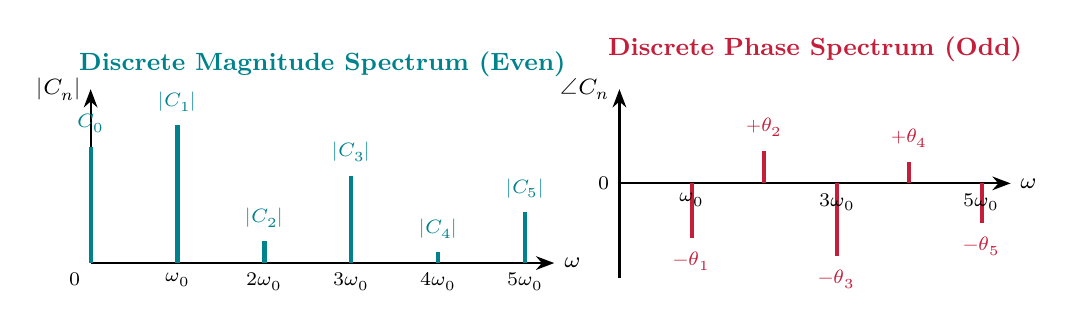
\begin{tikzpicture}[scale=0.92, auto]
  % Magnitude Spectrum
  \draw[-Stealth, thick] (0,0) -- (6.4,0) node[right, font=\footnotesize] {$\omega$};
  \draw[-Stealth, thick] (0,0) -- (0,2.4) node[left, font=\footnotesize] {$|C_n|$};
  \node[below left, font=\scriptsize] at (0,0) {$0$};
  
  \draw[line width=1.5pt, color=myteal] (0,0) -- (0,1.6) node[above=1pt, font=\scriptsize\bfseries] {$C_0$};
  \draw[line width=1.5pt, color=myteal] (1.2,0) -- (1.2,1.9) node[above=1pt, font=\scriptsize\bfseries] {$|C_1|$};
  \draw[line width=1.5pt, color=myteal] (2.4,0) -- (2.4,0.3) node[above=1pt, font=\scriptsize\bfseries] {$|C_2|$};
  \draw[line width=1.5pt, color=myteal] (3.6,0) -- (3.6,1.2) node[above=1pt, font=\scriptsize\bfseries] {$|C_3|$};
  \draw[line width=1.5pt, color=myteal] (4.8,0) -- (4.8,0.15) node[above=1pt, font=\scriptsize\bfseries] {$|C_4|$};
  \draw[line width=1.5pt, color=myteal] (6.0,0) -- (6.0,0.7) node[above=1pt, font=\scriptsize\bfseries] {$|C_5|$};
  
  \node[below, font=\scriptsize] at (1.2,0) {$\omega_0$};
  \node[below, font=\scriptsize] at (2.4,0) {$2\omega_0$};
  \node[below, font=\scriptsize] at (3.6,0) {$3\omega_0$};
  \node[below, font=\scriptsize] at (4.8,0) {$4\omega_0$};
  \node[below, font=\scriptsize] at (6.0,0) {$5\omega_0$};
  \node[font=\small\bfseries, color=myteal] at (3.2, 2.75) {Discrete Magnitude Spectrum (Even)};

  % Phase Spectrum (Shifted)
  \begin{scope}[shift={(7.3,1.1)}]
    \draw[-Stealth, thick] (0,0) -- (5.4,0) node[right, font=\footnotesize] {$\omega$};
    \draw[-Stealth, thick] (0,-1.3) -- (0,1.3) node[left, font=\footnotesize] {$\angle C_n$};
    \node[left, font=\scriptsize] at (0,0) {$0$};
    
    \draw[line width=1.5pt, color=myred] (1.0,0) -- (1.0,-0.75) node[below=1pt, font=\scriptsize\bfseries] {$-\theta_1$};
    \draw[line width=1.5pt, color=myred] (2.0,0) -- (2.0,0.45) node[above=1pt, font=\scriptsize\bfseries] {$+\theta_2$};
    \draw[line width=1.5pt, color=myred] (3.0,0) -- (3.0,-1.0) node[below=1pt, font=\scriptsize\bfseries] {$-\theta_3$};
    \draw[line width=1.5pt, color=myred] (4.0,0) -- (4.0,0.3) node[above=1pt, font=\scriptsize\bfseries] {$+\theta_4$};
    \draw[line width=1.5pt, color=myred] (5.0,0) -- (5.0,-0.55) node[below=1pt, font=\scriptsize\bfseries] {$-\theta_5$};
    
    \node[below, font=\scriptsize] at (1.0,0) {$\omega_0$};
    \node[below, font=\scriptsize] at (3.0,0) {$3\omega_0$};
    \node[below, font=\scriptsize] at (5.0,0) {$5\omega_0$};
    \node[font=\small\bfseries, color=myred] at (2.7, 1.85) {Discrete Phase Spectrum (Odd)};
  \end{scope}
\end{tikzpicture}
\end{tcolorbox}

% ───────────────────────────────────────────────────────────────────────────────
\section{Network Response to Non-Sinusoidal Periodic Inputs}
% ───────────────────────────────────────────────────────────────────────────────

\subsection{Harmonic Superposition Method}
When a linear time-invariant circuit is excited by a non-sinusoidal periodic voltage source:
\begin{equation}
  v(t) = V_0 + \sum_{n=1}^\infty V_{mn} \cos(n\omega_0 t + \theta_{vn})
\end{equation}
the steady-state current response is calculated by applying the \textbf{Superposition Principle} to each harmonic component independently.

\begin{tcolorbox}[formulabox, title={\textbf{Systematic Harmonic Solution Procedure}}]
\begin{enumerate}[leftmargin=*, itemsep=2pt, topsep=1pt]
  \item \textbf{DC Analysis ($n=0$):} Replace inductors with short circuits ($\mathbf{Z}_L = 0$) and capacitors with open circuits ($\mathbf{Z}_C = \infty$). Compute DC current:
  \begin{equation}
    I_0 = \frac{V_0}{R_{\text{eq}}}
  \end{equation}
  \item \textbf{$n$-th Harmonic Impedance:} Evaluate network input impedance at harmonic frequency $\omega_n = n\omega_0$:
  \begin{equation}
    \mathbf{Z}(j n \omega_0) = R_n + j X_n = |\mathbf{Z}_n| e^{j \phi_n} = |\mathbf{Z}_n| \angle \phi_n
  \end{equation}
  where inductive reactance scales directly ($X_{Ln} = n\omega_0 L$) and capacitive reactance scales inversely ($X_{Cn} = \frac{1}{n\omega_0 C}$).
  \item \textbf{$n$-th Harmonic Current Phasor:}
  \begin{equation}
    \mathbf{I}_{mn} = \frac{\mathbf{V}_{mn} \angle \theta_{vn}}{|\mathbf{Z}_n| \angle \phi_n} = \frac{V_{mn}}{|\mathbf{Z}_n|} \angle (\theta_{vn} - \phi_n) = I_{mn} \angle \theta_{in}
  \end{equation}
  \item \textbf{Total Time-Domain Current Synthesis:}
  \begin{equation}
    i(t) = I_0 + \sum_{n=1}^\infty I_{mn} \cos(n\omega_0 t + \theta_{vn} - \phi_n)
  \end{equation}
\end{enumerate}
\end{tcolorbox}

\subsection{Effective (RMS) Values and Average Power}

\begin{tcolorbox}[formulabox, title={\textbf{Formulas for RMS Values and Non-Sinusoidal Power}}]
\begin{itemize}[leftmargin=*, itemsep=3pt]
  \item \textbf{True RMS (Effective) Voltage and Current:}
  \begin{equation}
    V_{\text{rms}} = \sqrt{\frac{1}{T}\int_0^T v^2(t) dt} = \sqrt{V_0^2 + \sum_{n=1}^\infty \frac{V_{mn}^2}{2}} = \sqrt{V_0^2 + \sum_{n=1}^\infty V_{n,\text{rms}}^2}
  \end{equation}
  \begin{equation}
    I_{\text{rms}} = \sqrt{I_0^2 + \sum_{n=1}^\infty I_{n,\text{rms}}^2}
  \end{equation}
  \item \textbf{Total Average Active Power ($P$):} By orthogonality of distinct sinusoids over fundamental period $T$, all cross-harmonic terms integrate to zero:
  \begin{equation}
    P = \frac{1}{T}\int_0^T v(t) i(t) dt = V_0 I_0 + \sum_{n=1}^\infty V_{n,\text{rms}} I_{n,\text{rms}} \cos(\phi_n)
  \end{equation}
  \item \textbf{Apparent Power ($S$), Reactive Power ($Q$) and Distortion Power ($D$):}
  \begin{equation}
    S = V_{\text{rms}} I_{\text{rms}}, \qquad Q = \sum_{n=1}^\infty V_{n,\text{rms}} I_{n,\text{rms}} \sin(\phi_n), \qquad D = \sqrt{S^2 - P^2 - Q^2}
  \end{equation}
  \item \textbf{True Power Factor and Distortion Factor:}
  \begin{equation}
    \text{PF} = \frac{P}{S} = \frac{I_{1,\text{rms}}}{I_{\text{rms}}} \cdot \cos\phi_1 = (\text{Distortion Factor}) \times (\text{Displacement Factor})
  \end{equation}
  \item \textbf{Total Harmonic Distortion (THD):}
  \begin{equation}
    \text{THD}_I = \frac{\sqrt{\sum_{n=2}^\infty I_{n,\text{rms}}^2}}{I_{1,\text{rms}}} = \sqrt{\left(\frac{I_{\text{rms}}}{I_{1,\text{rms}}}\right)^2 - 1}
  \end{equation}
\end{itemize}
\end{tcolorbox}

% ───────────────────────────────────────────────────────────────────────────────
\section{The Continuous Spectrum via Fourier Transform}
% ───────────────────────────────────────────────────────────────────────────────

\begin{tcolorbox}[defbox, title={\textbf{Continuous Fourier Transform Pair}}]
As period $T \to \infty$, discrete spectral lines merge into a continuous density spectrum:
\begin{equation}
  X(j\omega) = \mathcal{F}\{x(t)\} = \int_{-\infty}^\infty x(t) e^{-j\omega t} dt
\end{equation}
\begin{equation}
  x(t) = \mathcal{F}^{-1}\{X(j\omega)\} = \frac{1}{2\pi} \int_{-\infty}^\infty X(j\omega) e^{j\omega t} d\omega
\end{equation}
\end{tcolorbox}
\par\vspace{4pt}\noindent
The \textbf{Energy Spectral Density} is $\mathcal{E}(\omega) = |X(j\omega)|^2$. Total signal energy is conserved under the transformation via \textbf{Parseval's Energy Theorem}:
\begin{equation}
  W = \int_{-\infty}^\infty |x(t)|^2 dt = \frac{1}{2\pi} \int_{-\infty}^\infty |X(j\omega)|^2 d\omega
\end{equation}

% ───────────────────────────────────────────────────────────────────────────────
\section{Three-Phase Unbalanced Circuits and Symmetrical Components}
% ───────────────────────────────────────────────────────────────────────────────

\subsection{Symmetrical Components Transformation (Fortescue's Theorem)}
In an unbalanced three-phase system, the three unsymmetrical phasor voltages or currents can be decomposed into three balanced symmetrical components:

\begin{tcolorbox}[defbox, title={\textbf{Fortescue's Theorem and the Complex Operator $a$}}]
Any set of three unbalanced phasors $\mathbf{V}_a, \mathbf{V}_b, \mathbf{V}_c$ can be uniquely expressed as the sum of three balanced symmetrical sets:
\begin{enumerate}[leftmargin=*, itemsep=2pt, topsep=1pt]
  \item \textbf{Positive-Sequence ($\mathbf{V}_{a1}, \mathbf{V}_{b1}, \mathbf{V}_{c1}$):} Equal magnitudes, $120^\circ$ phase separation, same phase sequence ($a$-$b$-$c$) as original.
  \item \textbf{Negative-Sequence ($\mathbf{V}_{a2}, \mathbf{V}_{b2}, \mathbf{V}_{c2}$):} Equal magnitudes, $120^\circ$ phase separation, reversed phase sequence ($a$-$c$-$b$).
  \item \textbf{Zero-Sequence ($\mathbf{V}_{a0}, \mathbf{V}_{b0}, \mathbf{V}_{c0}$):} Equal magnitudes and identical phase angles (in-phase).
\end{enumerate}
Defining the complex phase-shift operator $a = e^{j 120^\circ} = -\frac{1}{2} + j\frac{\sqrt{3}}{2}$:
\begin{equation}
  a^2 = e^{j 240^\circ} = -\frac{1}{2} - j\frac{\sqrt{3}}{2}, \qquad a^3 = 1, \qquad 1 + a + a^2 = 0
\end{equation}
\end{tcolorbox}

\begin{tcolorbox}[formulabox, title={\textbf{Matrix Transformation Relations}}]
The sequence components relate to the phase quantities by:
\begin{equation}
  \begin{bmatrix} \mathbf{V}_a \\ \mathbf{V}_b \\ \mathbf{V}_c \end{bmatrix}
  =
  \begin{bmatrix}
    1 & 1 & 1 \\
    1 & a^2 & a \\
    1 & a & a^2
  \end{bmatrix}
  \begin{bmatrix} \mathbf{V}_{a0} \\ \mathbf{V}_{a1} \\ \mathbf{V}_{a2} \end{bmatrix}
  = [\mathbf{A}] \mathbf{V}_{012}
\end{equation}
The inverse transformation matrix $[\mathbf{A}]^{-1}$ yields:
\begin{equation}
  \begin{bmatrix} \mathbf{V}_{a0} \\ \mathbf{V}_{a1} \\ \mathbf{V}_{a2} \end{bmatrix}
  = \frac{1}{3}
  \begin{bmatrix}
    1 & 1 & 1 \\
    1 & a & a^2 \\
    1 & a^2 & a
  \end{bmatrix}
  \begin{bmatrix} \mathbf{V}_a \\ \mathbf{V}_b \\ \mathbf{V}_c \end{bmatrix}
\end{equation}
Explicitly:
\begin{equation}
  \mathbf{V}_{a0} = \frac{\mathbf{V}_a + \mathbf{V}_b + \mathbf{V}_c}{3}, \quad \mathbf{V}_{a1} = \frac{\mathbf{V}_a + a\mathbf{V}_b + a^2\mathbf{V}_c}{3}, \quad \mathbf{V}_{a2} = \frac{\mathbf{V}_a + a^2\mathbf{V}_b + a\mathbf{V}_c}{3}
\end{equation}
\end{tcolorbox}

\begin{tcolorbox}[examplebox, title={\textbf{Physical Consequence: Zero-Sequence Current in Three-Phase Circuits}}]
In a three-phase system, the neutral current $\mathbf{I}_n$ is the sum of line currents:
\begin{equation}
  \mathbf{I}_n = \mathbf{I}_a + \mathbf{I}_b + \mathbf{I}_c = 3 \mathbf{I}_{a0}
\end{equation}
\textbf{Conclusion:}
\begin{itemize}[leftmargin=*, itemsep=2pt]
  \item In a 3-phase 3-wire system (ungrounded), $\mathbf{I}_a + \mathbf{I}_b + \mathbf{I}_c = 0 \implies \mathbf{I}_{a0} = 0$. Zero-sequence line current \textbf{cannot} flow in any 3-wire system.
  \item In delta-connected loads, line voltages sum to zero ($\mathbf{V}_{ab} + \mathbf{V}_{bc} + \mathbf{V}_{ca} = 0 \implies \mathbf{V}_{L0} = 0$), so zero-sequence voltage cannot exist across lines.
\end{itemize}
\end{tcolorbox}

\subsection{Neutral Shift Voltage (Millman's Theorem in 3-Phase Systems)}
When an unbalanced star-connected load with phase admittances $\mathbf{Y}_a, \mathbf{Y}_b, \mathbf{Y}_c$ is connected to a balanced source with neutral $N$, the star load neutral point $N'$ floats to a potential known as the \textbf{neutral shift voltage} $\mathbf{V}_{N'N}$:
\begin{equation}
  \mathbf{V}_{N'N} = \frac{\mathbf{V}_{AN} \mathbf{Y}_a + \mathbf{V}_{BN} \mathbf{Y}_b + \mathbf{V}_{CN} \mathbf{Y}_c}{\mathbf{Y}_a + \mathbf{Y}_b + \mathbf{Y}_c + \mathbf{Y}_n}
\end{equation}
where $\mathbf{Y}_n$ is the neutral wire admittance ($\mathbf{Y}_n = 0$ for 3-wire floating neutral). The voltage across each load branch is then $\mathbf{V}_{aN'} = \mathbf{V}_{AN} - \mathbf{V}_{N'N}$.

\subsection{Power Measurement by Two-Wattmeter Method}
The two-wattmeter method measures total active power in any 3-phase 3-wire system (balanced or unbalanced, star or delta):

\begin{tcolorbox}[tikzbox, title={\textbf{TikZ Schematic: Two-Wattmeter Connection in a Three-Phase System}}]
\centering
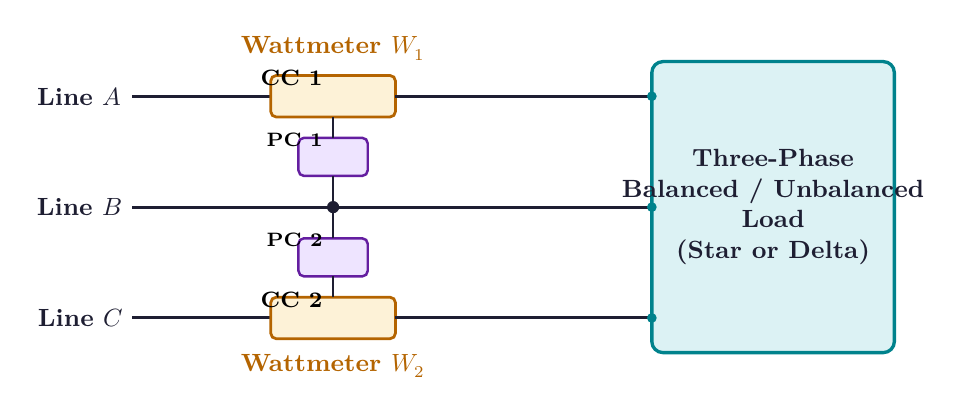
\begin{tikzpicture}[scale=0.88, auto]
  % 3 source lines
  \draw[line, line width=1.1pt] (0,2.6) node[left, font=\small\bfseries] {Line $A$} -- (2.0,2.6);
  \draw[line, line width=1.1pt] (0,1.0) node[left, font=\small\bfseries] {Line $B$} -- (7.5,1.0);
  \draw[line, line width=1.1pt] (0,-0.6) node[left, font=\small\bfseries] {Line $C$} -- (2.0,-0.6);

  % Wattmeter 1 (in Line A)
  \draw[fill=hdramber, draw=myamber, line width=1pt, rounded corners=2pt] (2.0,2.3) rectangle (3.8,2.9) node[midway, font=\footnotesize\bfseries] {CC 1};
  \draw[line, line width=1.1pt] (3.8,2.6) -- (7.5,2.6);
  \node[font=\small\bfseries, color=myamber, above=2pt] at (2.9,2.9) {Wattmeter $W_1$};

  \draw[fill=hdrpurple, draw=mypurple, line width=0.9pt, rounded corners=2pt] (2.4,1.45) rectangle (3.4,2.0) node[midway, font=\scriptsize\bfseries] {PC 1};
  \draw[line, thick] (2.9,2.3) -- (2.9,2.0);
  \draw[line, thick] (2.9,1.45) -- (2.9,1.0);

  % Wattmeter 2 (in Line C)
  \draw[fill=hdramber, draw=myamber, line width=1pt, rounded corners=2pt] (2.0,-0.9) rectangle (3.8,-0.3) node[midway, font=\footnotesize\bfseries] {CC 2};
  \draw[line, line width=1.1pt] (3.8,-0.6) -- (7.5,-0.6);
  \node[font=\small\bfseries, color=myamber, below=2pt] at (2.9,-0.9) {Wattmeter $W_2$};

  \draw[fill=hdrpurple, draw=mypurple, line width=0.9pt, rounded corners=2pt] (2.4,0.0) rectangle (3.4,0.55) node[midway, font=\scriptsize\bfseries] {PC 2};
  \draw[line, thick] (2.9,-0.3) -- (2.9,0.0);
  \draw[line, thick] (2.9,0.55) -- (2.9,1.0);

  % Solder junction on Line B
  \fill[mydark] (2.9,1.0) circle (2.5pt);

  % Load block
  \draw[fill=hdrteal, draw=myteal, line width=1.2pt, rounded corners=4pt] (7.5,-1.1) rectangle (11.0,3.1);
  \node[align=center, font=\small\bfseries, color=mydark] at (9.25,1.0) {Three-Phase\\Balanced / Unbalanced\\Load\\(Star or Delta)};

  % Connection terminals to Load
  \fill[myteal] (7.5,2.6) circle (2pt);
  \fill[myteal] (7.5,1.0) circle (2pt);
  \fill[myteal] (7.5,-0.6) circle (2pt);
\end{tikzpicture}
\end{tcolorbox}

\begin{tcolorbox}[formulabox, title={\textbf{Two-Wattmeter Power and Power Factor Relations}}]
Under balanced sinusoidal conditions with line-to-line voltage $V_L$, line current $I_L$, and load power factor angle $\phi$:
\begin{equation}
  W_1 = V_L I_L \cos(30^\circ - \phi), \qquad W_2 = V_L I_L \cos(30^\circ + \phi)
\end{equation}
\begin{enumerate}[leftmargin=*, itemsep=2pt, topsep=1pt]
  \item \textbf{Total Active Power ($P$):}
  \begin{equation}
    P = W_1 + W_2 = V_L I_L [\cos(30^\circ - \phi) + \cos(30^\circ + \phi)] = \sqrt{3} V_L I_L \cos\phi
  \end{equation}
  \item \textbf{Total Reactive Power ($Q$):}
  \begin{equation}
    W_1 - W_2 = V_L I_L [\cos(30^\circ - \phi) - \cos(30^\circ + \phi)] = V_L I_L \sin\phi \implies Q = \sqrt{3}(W_1 - W_2)
  \end{equation}
  \item \textbf{Power Factor Angle ($\phi$):}
  \begin{equation}
    \tan\phi = \sqrt{3} \frac{W_1 - W_2}{W_1 + W_2} \implies \text{PF} = \cos\phi = \cos\left[ \tan^{-1}\left( \sqrt{3}\frac{W_1 - W_2}{W_1 + W_2} \right) \right]
  \end{equation}
\end{enumerate}
\end{tcolorbox}

\newpage
% ===============================================================================
% MANDATORY QUICK REVISION PAGE
% ===============================================================================
\begin{center}
  {\large\bfseries\color{myred} Quick Revision --- Module 2}\\[3pt]
  {\small\color{mydark} Fourier Analysis and Three-Phase Unbalanced Systems $|$ EC304}
\end{center}
\noindent{\color{myred}\rule{\linewidth}{1.2pt}}
\vspace{4pt}

\begin{tcolorbox}[formulabox, title={\textbf{Key Formulas and Network Relations at a Glance}}]
\renewcommand{\arraystretch}{1.35}
\begin{tabularx}{\linewidth}{B{5.0cm} X}
Trigonometric Fourier Form & $f(t) = a_0 + \sum_{n=1}^\infty [a_n \cos(n\omega_0 t) + b_n \sin(n\omega_0 t)]$ \\[4pt]
Exponential Fourier Form & $f(t) = \sum_{n=-\infty}^\infty C_n e^{j n \omega_0 t}, \quad C_n = \frac{a_n - j b_n}{2}$ \\[4pt]
True RMS Voltage & $V_{\text{rms}} = \sqrt{V_0^2 + \sum_{n=1}^\infty V_{n,\text{rms}}^2}$ \\[4pt]
Average Non-Sinusoidal Power & $P = V_0 I_0 + \sum_{n=1}^\infty V_{n,\text{rms}} I_{n,\text{rms}} \cos(\phi_n)$ \\[4pt]
True Power Factor & $\text{PF} = \frac{P}{S} = \frac{I_{1,\text{rms}}}{I_{\text{rms}}} \cos\phi_1$ \\[4pt]
Total Harmonic Distortion & $\text{THD} = \frac{\sqrt{\sum_{n=2}^\infty I_{n,\text{rms}}^2}}{I_{1,\text{rms}}}$ \\[4pt]
Complex Operator $a$ & $a = e^{j 120^\circ} = -\frac{1}{2} + j\frac{\sqrt{3}}{2}, \quad 1 + a + a^2 = 0$ \\[4pt]
Zero-Sequence Current & $\mathbf{I}_{a0} = \frac{\mathbf{I}_a + \mathbf{I}_b + \mathbf{I}_c}{3} = \frac{\mathbf{I}_n}{3}$ \\[4pt]
Two-Wattmeter Total Power & $P_{\text{total}} = W_1 + W_2 = \sqrt{3} V_L I_L \cos\phi$ \\[4pt]
Two-Wattmeter Power Factor & $\tan\phi = \sqrt{3} \frac{W_1 - W_2}{W_1 + W_2}$ \\[4pt]
\end{tabularx}
\end{tcolorbox}

\begin{tcolorbox}[defbox, title={\textbf{One-Line Definitions}}]
\begin{itemize}[leftmargin=*, itemsep=2pt, topsep=0pt]
  \item \textbf{Harmonic Frequency:} An integer multiple ($n\omega_0$) of the fundamental repetition frequency of a periodic wave.
  \item \textbf{Half-Wave Symmetry:} Condition $f(t \pm T/2) = -f(t)$, ensuring complete cancellation of all even harmonic orders.
  \item \textbf{Line Spectrum:} A discrete graphical plot of harmonic component amplitudes and phase shifts versus frequency.
  \item \textbf{Harmonic Impedance:} The frequency-dependent impedance of a circuit evaluated specifically at harmonic frequency $n\omega_0$.
  \item \textbf{Distortion Power ($D$):} The component of apparent power caused strictly by harmonic cross-frequencies, measured in VA.
  \item \textbf{Displacement Factor:} The cosine of the fundamental phase angle ($\cos\phi_1$), measuring fundamental displacement.
  \item \textbf{Symmetrical Components:} Three balanced phasor sets (positive, negative, zero) replacing an unbalanced three-phase system.
  \item \textbf{Neutral Shift Voltage:} The potential difference appearing between floating load neutral and source star neutral in unbalanced loads.
  \item \textbf{Two-Wattmeter Method:} A standard method using two power meters to measure total power in any three-phase three-wire system.
  \item \textbf{Parseval's Theorem:} Mathematical relation stating total energy is conserved between time and continuous frequency domains.
\end{itemize}
\end{tcolorbox}

\begin{tcolorbox}[exambox, title={\textbf{Frequently Asked / Viva Questions}}]
\begin{enumerate}[topsep=0pt, label=\textbf{Q\arabic*.}, itemsep=5pt]
  \item \Q{What harmonics are present in a periodic waveform possessing Half-Wave Symmetry?}
  A waveform with half-wave symmetry ($f(t \pm T/2) = -f(t)$) contains strictly odd harmonics ($n = 1, 3, 5, \dots$). The DC component ($a_0$) and all even harmonics ($a_{2k}, b_{2k}$) are identically zero.

  \item \Q{Why does a non-sinusoidal voltage produce an active power contribution only with currents of the identical harmonic order?}
  Because the time-average product of two sinusoids of differing frequencies over the fundamental period is identically zero: $\int_0^T \cos(m\omega_0 t)\cos(n\omega_0 t)dt = 0$ for $m \ne n$. Active power is generated exclusively by voltage and current terms belonging to the same harmonic frequency.

  \item \Q{Can zero-sequence currents flow in a balanced or unbalanced 3-phase 3-wire system? Explain.}
  No. In any 3-phase 3-wire system, by KCL, the sum of line currents must be zero ($\mathbf{I}_a + \mathbf{I}_b + \mathbf{I}_c = 0$). Since zero-sequence current is $\mathbf{I}_{a0} = \frac{1}{3}(\mathbf{I}_a + \mathbf{I}_b + \mathbf{I}_c)$, it is strictly zero. A neutral or ground path is required for zero-sequence current to exist.

  \item \Q{What does it mean if one wattmeter reads negative in the two-wattmeter method?}
  A negative reading occurs when the load power factor is less than $0.5$ ($\phi > 60^\circ$). In that case, $W_2 = V_L I_L \cos(30^\circ + \phi)$ becomes negative. Total power is still the algebraic sum $W_1 + W_2$.

  \item \Q{What are the readings of the two wattmeters at unity power factor ($\cos\phi = 1$)?}
  At unity power factor, $\phi = 0^\circ$. Thus, $W_1 = V_L I_L \cos(30^\circ) = \frac{\sqrt{3}}{2}V_L I_L$ and $W_2 = V_L I_L \cos(30^\circ) = \frac{\sqrt{3}}{2}V_L I_L$. Both wattmeters read identical positive values ($W_1 = W_2 = P/2$).

  \item \Q{What are the readings of the two wattmeters at zero power factor ($\cos\phi = 0$)?}
  At zero power factor, $\phi = 90^\circ$. Then $W_1 = V_L I_L \cos(-60^\circ) = 0.5 V_L I_L$ and $W_2 = V_L I_L \cos(120^\circ) = -0.5 V_L I_L$. The wattmeters have equal magnitudes but opposite signs ($W_1 = -W_2$), yielding net active power $P = W_1 + W_2 = 0$.

  \item \Q{State the relationship between Total Harmonic Distortion (THD) and Distortion Factor.}
  The distortion factor $\mu = I_{1,\text{rms}} / I_{\text{rms}}$ relates to THD by $\mu = \frac{1}{\sqrt{1 + \text{THD}^2}}$. As harmonic distortion increases, the distortion factor decreases below unity, degrading true power factor.

  \item \Q{What is the physical meaning of the complex operator $a = e^{j 120^\circ}$?}
  The operator $a$ represents a counter-clockwise phase rotation of $120^\circ$ ($2\pi/3\text{ radians}$) without altering the magnitude of the phasor. Multiplying by $a^2$ rotates by $240^\circ$.

  \item \Q{How does Millman's Theorem find the neutral shift in an unbalanced 3-phase star circuit?}
  Millman's theorem treats the 3 phase voltages as parallel branches connected to neutral. The star point voltage is $\mathbf{V}_{N'N} = (\sum \mathbf{V}_k \mathbf{Y}_k) / \sum \mathbf{Y}_k$, directly yielding the shift in neutral potential.

  \item \Q{Distinguish between continuous and discrete Fourier spectra.}
  A discrete spectrum consists of isolated impulses at integer multiples of fundamental frequency $n\omega_0$, characteristic of periodic signals. A continuous spectrum is a continuous function of $\omega$ spanning all frequencies, characteristic of non-periodic transient energy pulses.
\end{enumerate}
\end{tcolorbox}

\begin{tcolorbox}[tikzbox, title={\textbf{Summary Matrix: Waveform Symmetries and Two-Wattmeter Diagnostic Rules}}]
\par\vspace{4pt}\noindent
\begingroup
\setlength{\tabcolsep}{4.5pt}
\setlength{\extrarowheight}{3pt}
\renewcommand{\arraystretch}{1.35}
\begin{tabularx}{\linewidth}{|B{3.2cm}|B{3.8cm}|Y|}
\hline
\multicolumn{1}{|c|}{\textbf{Operating Condition}} & \multicolumn{1}{c|}{\textbf{Wattmeter Relationship}} & \multicolumn{1}{c|}{\textbf{Power Factor / Significance}} \\
\hline
$\phi = 0^\circ$ (Resistive) & $W_1 = W_2 > 0$ & $\text{PF} = 1.0$; identical positive readings. \\
\hline
$\phi = 60^\circ$ & $W_1 > 0, \quad W_2 = 0$ & $\text{PF} = 0.5$; meter 2 reads exactly zero. \\
\hline
$\phi > 60^\circ$ (Lagging) & $W_1 > 0, \quad W_2 < 0$ & $\text{PF} < 0.5$; meter 2 reverses deflection. \\
\hline
$\phi = 90^\circ$ (Pure Reactive) & $W_1 = -W_2$ & $\text{PF} = 0$; net active power is strictly zero. \\
\hline
Unbalanced 3-Wire System & $W_1 + W_2 = P_{\text{total}}$ & Valid regardless of load unbalance or power factor. \\
\hline
\end{tabularx}
\endgroup
\end{tcolorbox}

\end{document}
